\documentclass{article}
\usepackage[utf8]{inputenc}
\usepackage{graphicx}
\usepackage{amsmath}
\usepackage[a4paper, total={8in, 11in}]{geometry}
\setlength\parindent{0pt}
\begin{document}
\textbf{Back references: refers to the exact part of string that is matched to the group number not matched to the pattern \\}
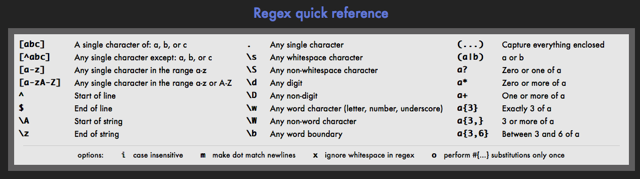
\includegraphics[width=4cm,height =3cm]{regexTable.jpg}
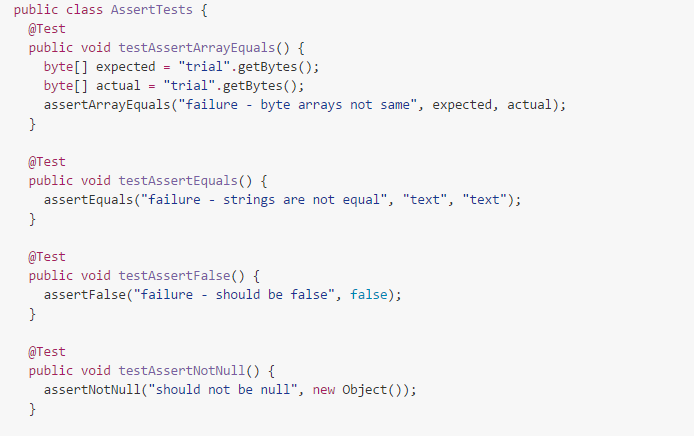
\includegraphics[width=6cm,height =3cm]{testCases.png}\\
\textbf{UML Design Patterns}\\
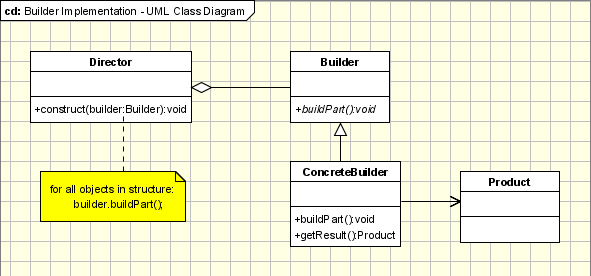
\includegraphics[width=6cm,height =3cm]{builder.png}
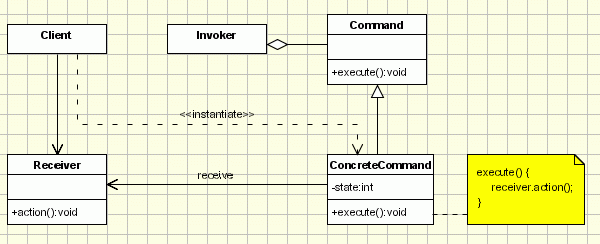
\includegraphics[width=6cm,height =3cm]{command.png}
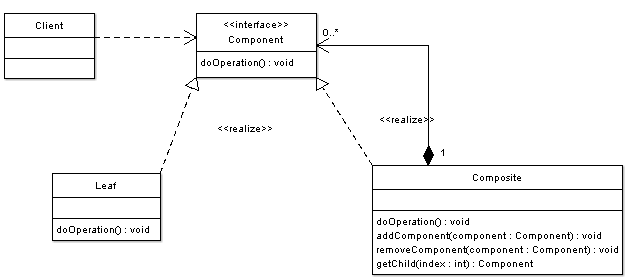
\includegraphics[width=6cm,height =3cm]{composite.png}\\
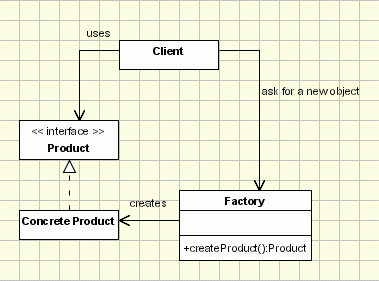
\includegraphics[width=6cm,height =3cm]{factory.png}
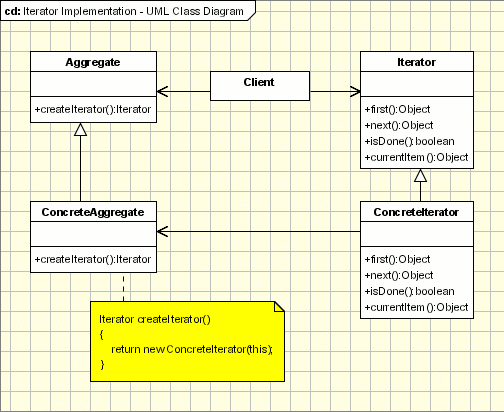
\includegraphics[width=6cm,height =3cm]{it.png}
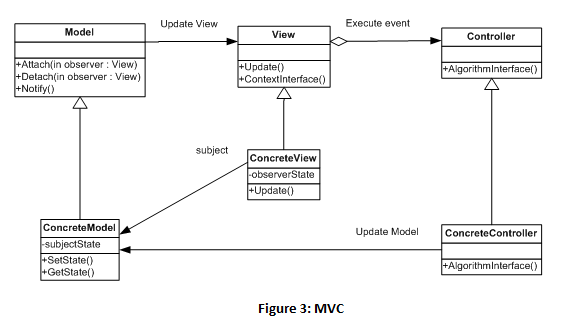
\includegraphics[width=6cm,height =3cm]{mvc.png}\\
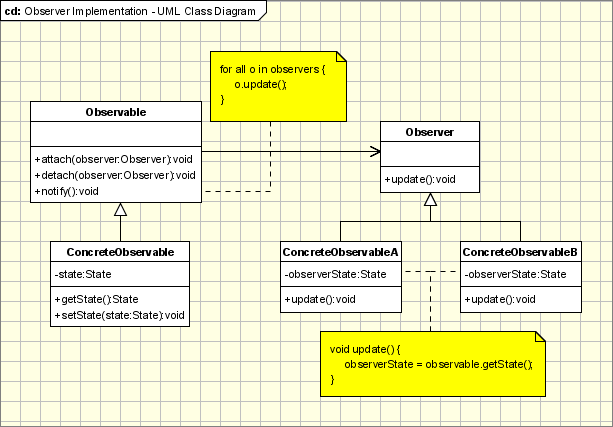
\includegraphics[width=6cm,height =3cm]{obs.png}
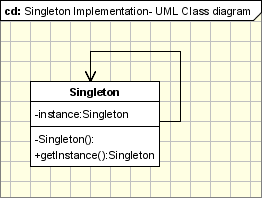
\includegraphics[width=6cm,height =3cm]{singleton.png}
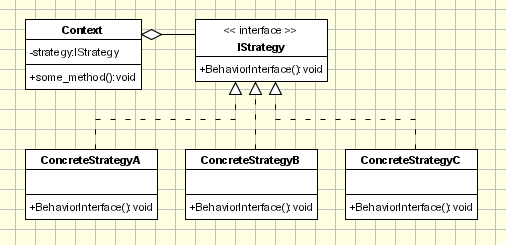
\includegraphics[width=6cm,height =3cm]{strategy.png}\\
\textbf{Git Basics}
git pull [location name]\\
git add [file name] or . (adds all)\\
git commit -m (message)\\
git push [file name]\\
git checkout [branch name] -- switches branches\\
git branch [branch name] -- creates new branch or checks which branches exist.\\
git log -- shows log of past push history\\
git clone [location]\\
git merge [file name] \\
git branch -D [branch] Force delete the specified branch\\
git branch -d [branch] Delete the specified branch. prevents you from deleting the branch if it has unmerged changes.\\
git branch -m [branchName] rename branch to branchName\\
Dealing with merge conflict, run the git status command shows you which files need to be resolved, Fix these files, then git add, then commit and push as usual\\

\begin{verbatim}
public class fileParser(){
    private Pattern pname = Pattern.compile("regex");
    public boolean parse(BufferReader input){
    try{int state 0; Matcher m; String L;
        while((L = input.readLine()) != null) {
            switch(state){
                case 0:
                    m = pname.matcher(L);
                    if(m.matches()){int p1 = Integer.parseInt(m.group(1));state = 1; break;}
                    error("message";
                    return false;
                }#state
            }#while
        }#try
        catch(Exception e){}
        return true;
    }#method
}#class				
\end{verbatim}
\textbf{Inheritance}\\
In a subclass:\\
-use super.attribute to refer to a variable or method in parent class\\
-use super(attribute) to call a constructor defined in parent class\\
\begin{verbatim}
public class LandAnimal extends Animal{
    public LandAnimal(String name){super(name);}}
\end{verbatim}
\textbf{UML}\\
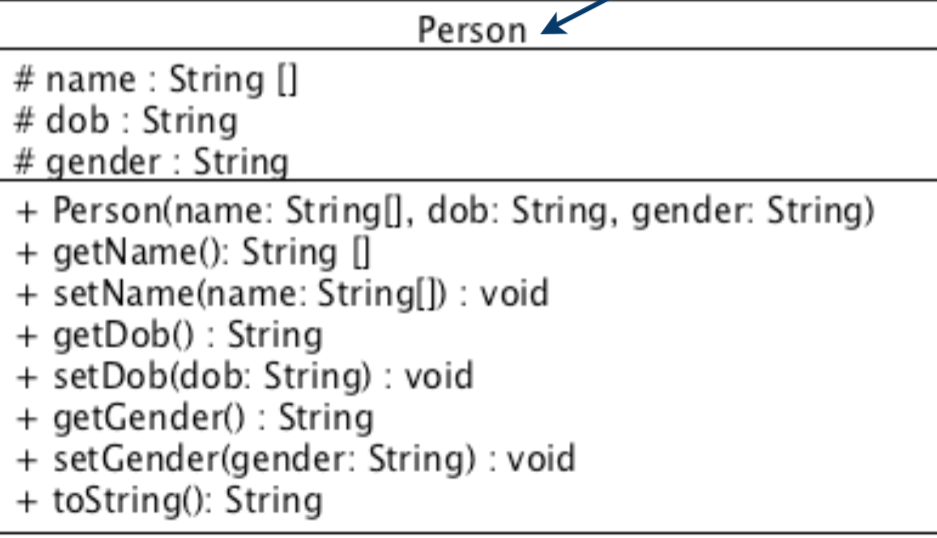
\includegraphics[width=6cm,height =3cm]{umlexample.png}
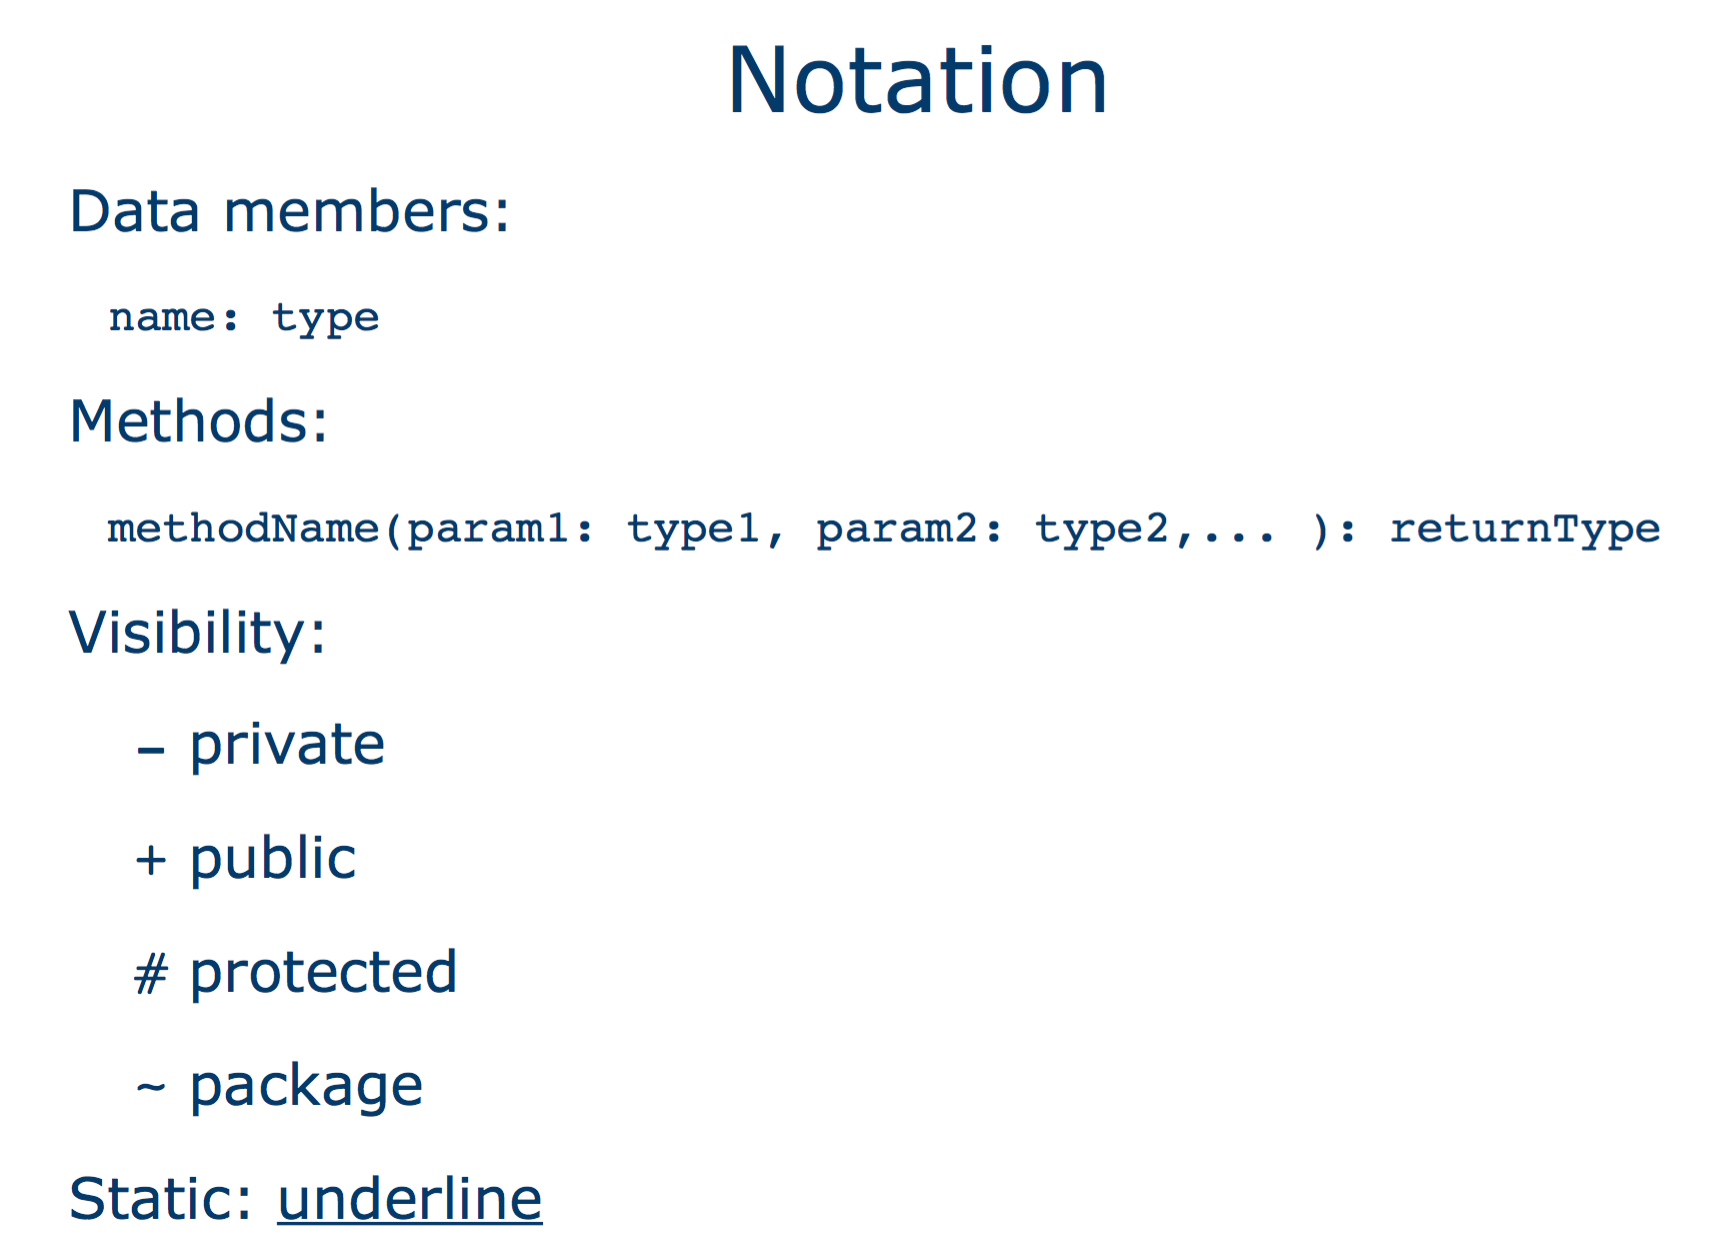
\includegraphics[width=6cm,height =3cm]{notation.png}
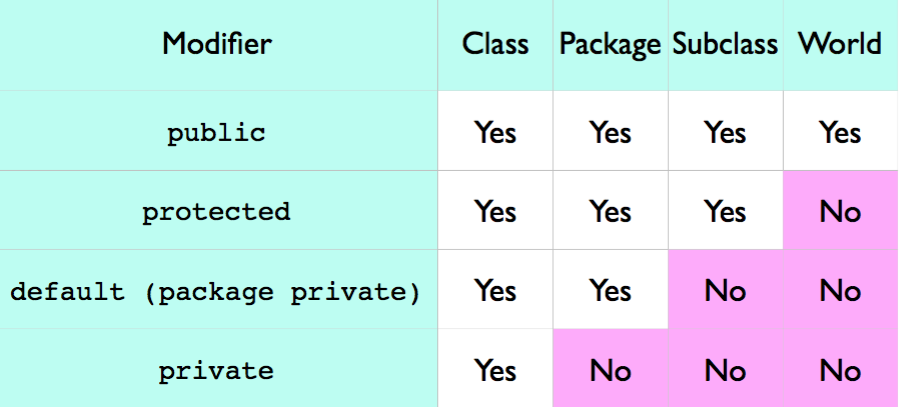
\includegraphics[width=6cm,height =3cm]{table.png}\\

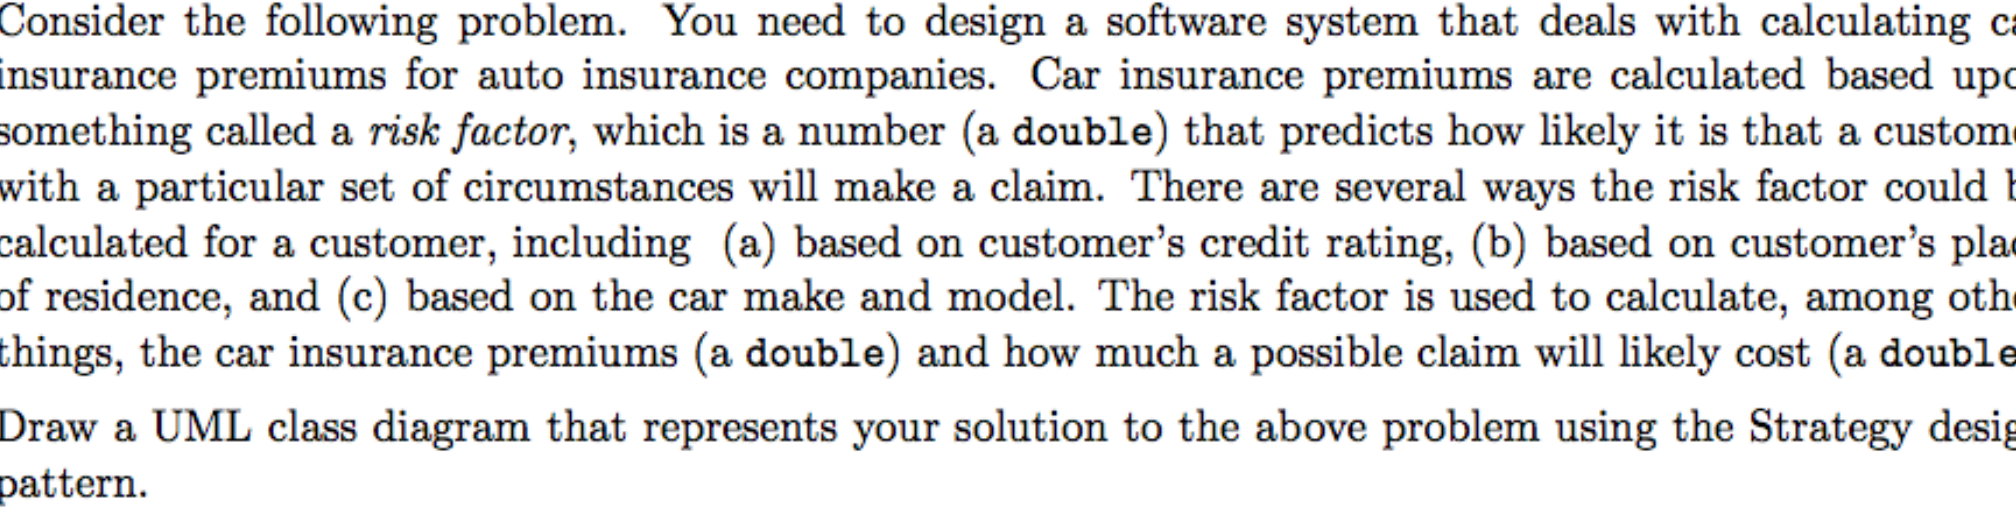
\includegraphics[width=7cm,height =3cm]{Riskq.png}
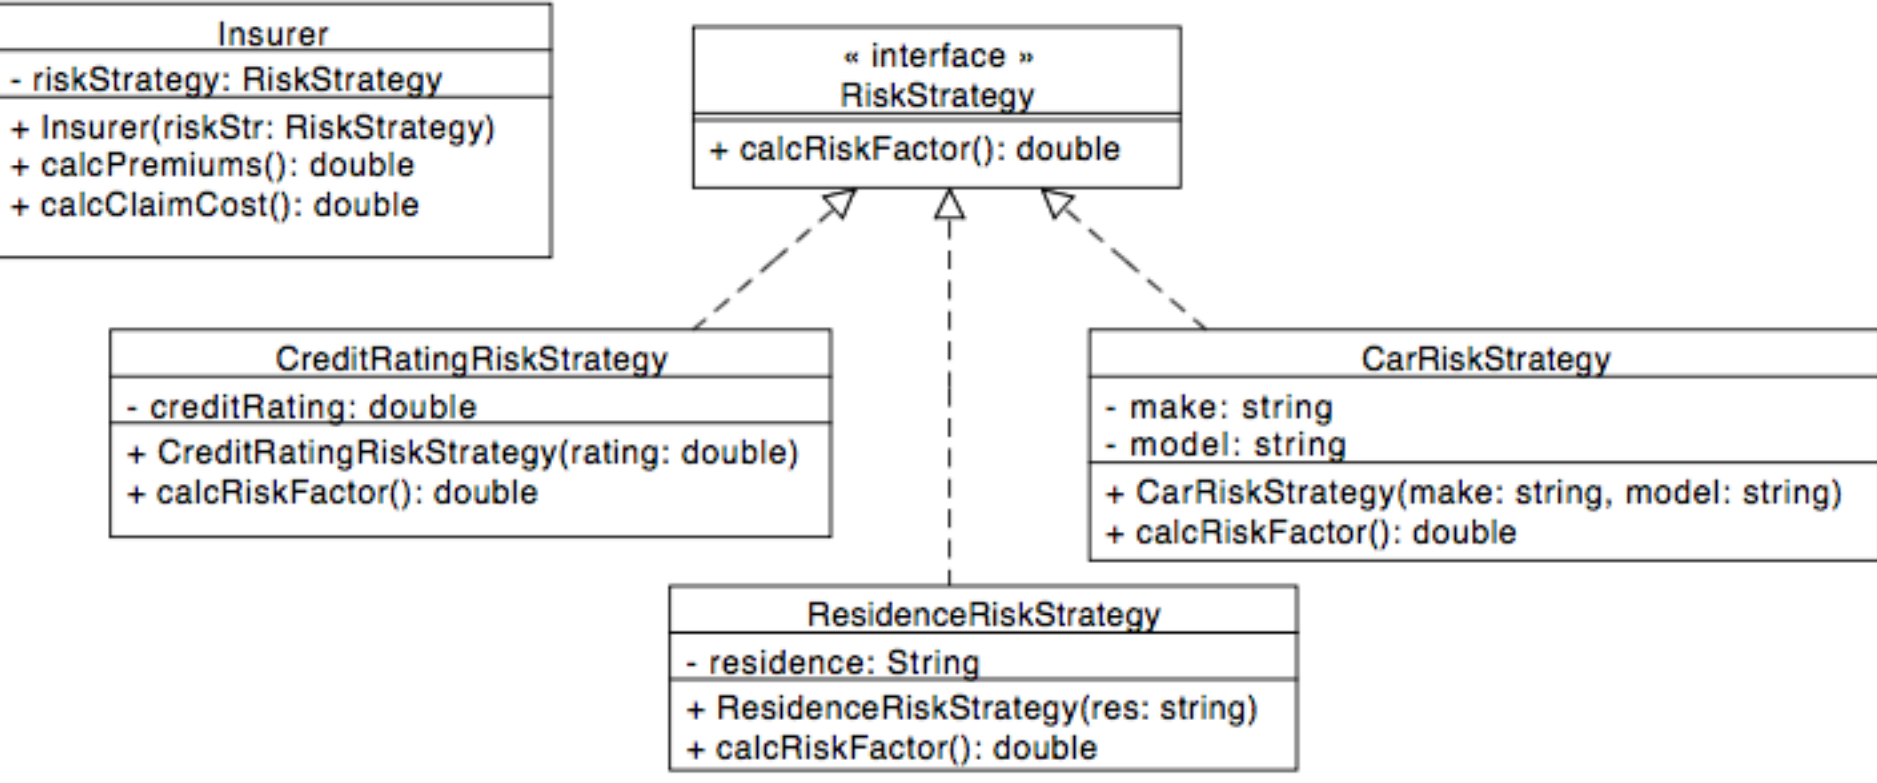
\includegraphics[width=8cm,height =3cm]{Riskuml.png}\\
\textbf{Iterator}
\begin{verbatim}
public class SongsMain {
    public static void main(String[] args) {
        YourSongs songs1 = new YourSongs(); #iterable
        Iterator<Song> it = songs1.iterator(); #iterator
		while (it.hasNext()) {it.next();}}}  
public class YourSongs implements Iterable<Song> {
    Song[] songs;
    public YourSongs() {songs = new Song[1];songs[0] = new Song("Hello", "Adele");}
    public Iterator<Song> iterator() {return new YourSongsIterator(songs);}}
public class YourSongsIterator implements Iterator<Song> {
    private Song[] songs; // HashMap<Integer, Song> songs;
    private int indexKey;
    public YourSongsIterator(Song[] s) {this.songs = s; indexKey = 0;}
	public boolean hasNext() {return this.indexKey < this.songs.length;}
    public Song next() {return this.songs[indexKey++];}}

\end{verbatim}
\textbf{Builder Design Pattern Example}
\begin{verbatim}
public static void main(String[] args){
    Director director = new Director();
    Builder builder = Null;
    Scanner s = new Scanner(System.in);
    String ans = s.nextline();
    if(ans.equals("kid"){builder = new Kidsmealbuilder();}
    else{builder = new Studentmealbuilder();}
    Meal meal = director.createMeal(builder)}
public abstract class MealBuilder {
    protected Meal meal = new Meal();	
    public abstract void buildDrink();
    public abstract void buildMain();
    public abstract Meal getMeal();}
public class director{
    #no constructor
    public Meal createMeal(Mealbuilder builder){ builder.buildDrink(); builder.buildFood();
    return builder.getMeal();}
public class KidsMealBuilder extends MealBuilder{
    public void buildDrink(){meal.setDrink("Kid drink: Kool-aid");}
    public void buildMain(){meal.setMain("Chicken nuggets");}
    public Meal getMeal(){return meal;}
\end{verbatim}
\textbf{Singleton}
\begin{verbatim}
public class Client(){
        Singleton S1 = Singleton.getInstance();
        Singleton S2 = Singleton.getInstance(); #S1 and S2 are the same instance of the singleton object}
public class Singleton(){
    private static Singleton instance = new Singleton();
    public static Singleton getInstance() {
        return instance;}}
\end{verbatim}
\textbf{Command}
\begin{verbatim}
public class Client(){
    Receiver R = new Receiver();
    Invoker = I = new Invoker();
    Command C = new concreteCommand(Receiver R);
    invoker.setCommand(C);
    invoker.execute();
public class concreteCommand implements Command {
    Light light;
    public TurnOffCommand(Light light) {this.light = light;}
    public void execute() {this.light.switchOff();}}
\end{verbatim}
\textbf{Composite}
\begin{verbatim}
public interface GraphicComponent{public void paint();}
public class SimpleGraphic implements GraphicComponent {
    public void paint() {System.out.println("I am a simple graphic.");}}
public class CompositeGraphic implements GraphicComponent {
    ArrayList<GraphicComponent> graphics = new ArrayList<>();
    public void paint() {
        for (GraphicComponent g: graphics){g.paint();}}
        public void add(GraphicComponent g) {graphics.add(g);}
        public void remove(GraphicComponent g) {graphics.remove(g);}}
public class Client{
    public static void main(String[] args) {
        SimpleGraphic graphic1 = new SimpleGraphic();
        CompositeGraphic graphicGroup1 = new CompositeGraphic();
        graphicGroup1.add(graphic1);
        CompositeGraphic mainGroup = new CompositeGraphic();
        mainGroup.add(graphicGroup1);
        mainGroup.paint();}}
\end{verbatim}
\textbf{Strategy}
\begin{verbatim}
public interface TravelStrategy {
    public void travel(Person p, String location);}
public class CarStrategy implements TravelStrategy {
    public void travel(Person p, String location) {
        p.setLocation(location);
        System.out.println(p.getName() + " has traveled to " + p.getLocation() + " by car.");}}
public class TravelContext {
    private TravelStrategy strategy;
    public void setTravelStrategy(TravelStrategy s){strategy =s;}
    public void takeTrip(Person p, String location) {strategy.travel(p, location);}}
public class Client {
    public static void main(String[] args) {
        TravelContext ctx = new TravelContext();
        ctx.setTravelStrategy(new BusStrategy());
        ctx.takeTrip(new Person("Sadia", "Canada"), "Australia");}}
\end{verbatim}
\textbf{Factory}
\begin{verbatim}
public class Main {
    public static void main(String[] args) {
        Fruit fruit;
        FruitFactory fruitFactory = new FruitFactory();
        fruit = fruitFactory.makeFruit("Apple");
        fruit = fruitFactory.makeFruit("Orange");}}
public class FruitFactory {
    public Fruit makeFruit(String type) {
        Fruit fruit = null;
        if (type == "Apple") {fruit = new Apple();}
        else if (type == "Orange") {fruit = new Orange();}
        return fruit;}}
public abstract class Fruit {
    final String type;
    public Fruit(String type){this.type = type;}
    public String getType() {return type;}}
public class Apple extends Fruit {
    public Apple() {super("Apple");}}
\end{verbatim}
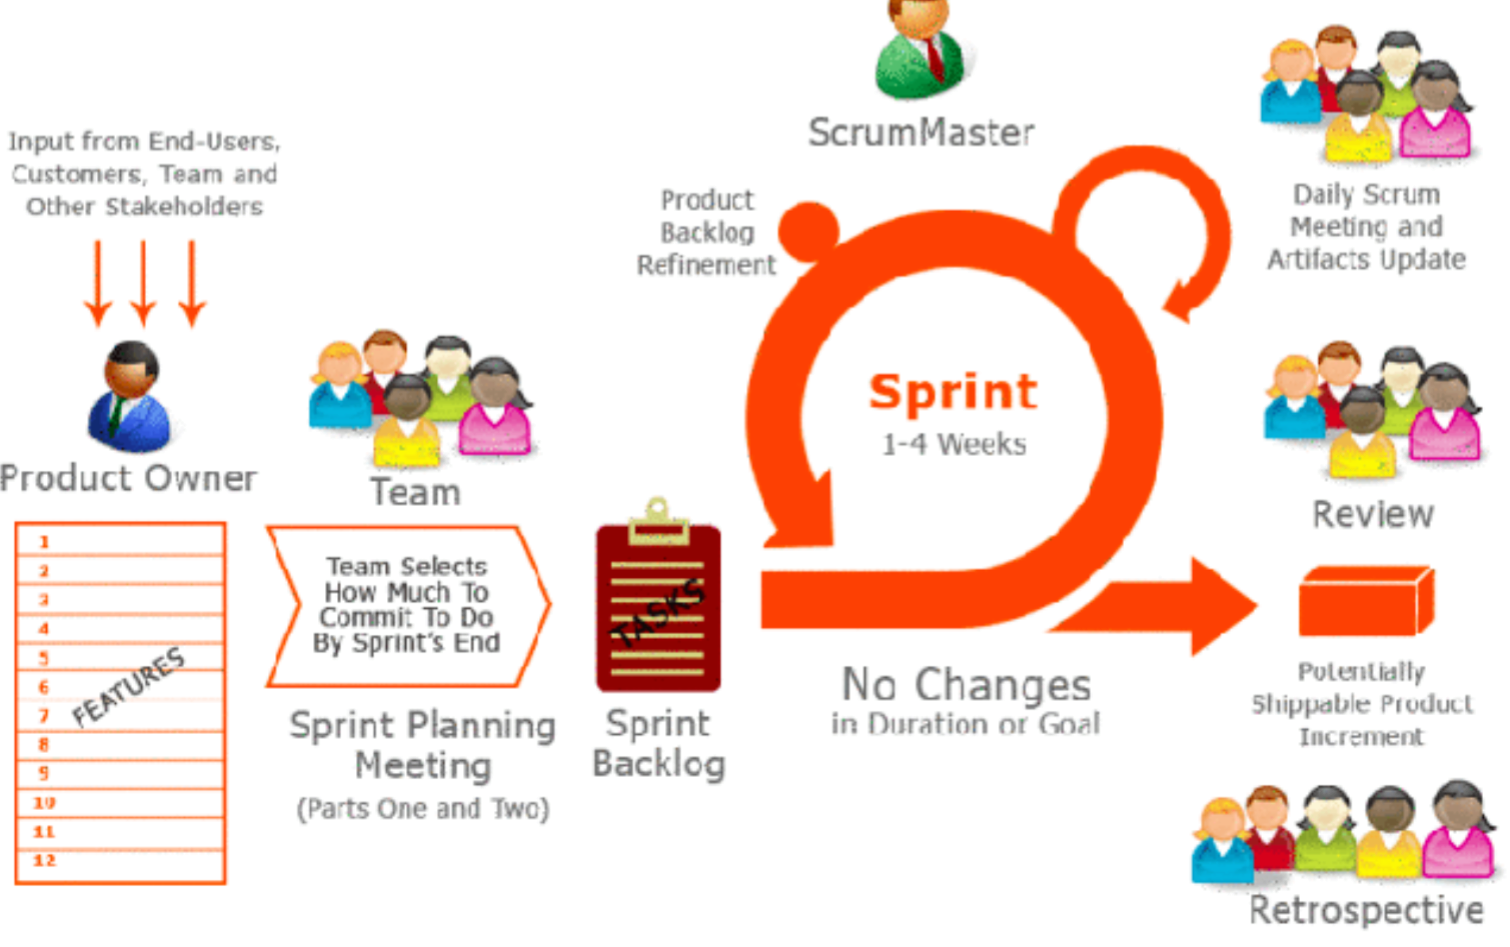
\includegraphics[width=6cm,height =4.5cm]{scrum.png}\\
Product Owner: Responsible for product backlog, represents users, expresses backlog items and orders them by value \\
Development Team: Responsible for delivering potentially shippable increment of working software \\
Scrum Master: Removes obstacles, facilitates scrum events and communication \\
Product Backlog: Source of requirements for any changes to be made to the product. Ordered by value, risk, priority and necessity, estimated by team
Sprint planning meeting: Team selects items from backlog and defines a sprint goal, and the items are converted into tasks and estimated \\
Daily Scrum Meeting: Short meeting for the team to discuss what has been accomplished since last meeting, what will be done before the next meeting, and what obstacles are in the way \\
Sprint Review: Product Owner identifies what has been done, team discusses development process and demos current increment of software, product owner discusses current state of backlog, team decides what to do next \\

\textbf{IEEE Conversion}\\
   $ \underbrace{0}_\texttrm{+/-}  \underbrace{01111110}_\texttrm{8 bit reps exponent + 127}  \underbrace{01000000000000000000000}_\texttrm{23 bit mantissa}$\\

   
\textbf{Rounding GRS}\\ 
0xx - round down/do nothing\\
100 - round up if mantissa's bit just before G is 1, else round down/do nothing.\\
101/110/111 - round up\\
Rounding up is done by adding 1 to the mantissa in the mantissa's least significant bit position just before G. G is the 1st element after the 23 mantissa.\\
\textbf{Example for float -6.8}\\
6: 2^2 + 2^ 1 + 2^0 <=> 110\\\\
0.8: 1100...
$
\begin{array}{cc}
  \{ & 
    \begin{array}{cc}
      0.8*2 & =\textbf{1}.6 \\
      0.6*2 & =\textbf{1}.2 \\
      0.2*2 & =\textbf{0}.4 \\
      0.4*2 & =\textbf{0}.8 \\
    \end{array}
\end{array}
$\\\\
$
mantissa = 110.1100 1100 1100 1100 1100 1 (24 since you don't count the first one)\\
Normalize mantissa to find exponent: 1.10(.)110011001100110011001 * 2^2$ (Shifted 2 decimal places so exponent is 2)\\

8 bit exponent: Binary of (127 + exponent value) = 127 + 2 = 129 = 2^7 + 2^0 <=> 10000001\\\\
\textbf{The IEEE is: }\\\\
$ \underbrace{1}_\texttrm{Since Negative}  \underbrace{10000001}_\texttrm{129 bin rep}  \underbrace{10110011001100110011001}_\texttrm{23 bit mantissa}$\\\\
Round up since GRS is 100 and the element before G is a 1. Since 001 represents 1 in binary, and 1+1 = 2, the resulting binary rep is 010.\\
Final IEEE:  {$ \underbrace{1}_\texttrm{ }  \underbrace{10000001}_\texttrm{8 bit}  \underbrace{10110011001100110011010}_\texttrm{23 bit mantissa}$}\\
Note: Interfaces can extend other interfaces, classes can implement multiple interfaces, classes can only extend a single class
Note: Abstract classes cannot be instantiated
Note: If A extends B, then the code {A a = new B();} is valid but the code {B b = new A();} is invalid because of a type mismatch




\end{document}